\section{Serial Data Transfer}

\subsection{Serial Communication Basics}

\mult{2}

\begin{concept}{Serial vs. Parallel Communication}\\
Microcontrollers often use serial connections for communication:

\textbf{Serial Connection}: Data transmitted one bit at a time over fewer wires
    \begin{itemize}
        \item Simpler (saves PCB area)
        \item Reduces number of switching lines (reduced power, improved EMC)
        \item Requires higher-level protocol for interpretation
    \end{itemize}
\textbf{Parallel Bus}: Data transmitted over multiple lines simultaneously
    \begin{itemize}
        \item Faster for short distances
        \item More complex routing
        \item Higher power consumption and EMC issues
    \end{itemize}
\end{concept}

\begin{definition}{Serial Communication Modes}
\begin{itemize}
    \item \textbf{Simplex}: Unidirectional, one-way only communication
    \item \textbf{Half-duplex}: Bidirectional, but only one direction at a time
    \item \textbf{Full-duplex}: Bidirectional, both directions simultaneously
\end{itemize}
\end{definition}

\begin{definition}{Serial Communication Timing}

    \textbf{Synchronous}: Both nodes use the same clock
    \begin{itemize}
        \item Clock often provided by master
        \item Examples: SPI, I2C
    \end{itemize}
\textbf{Asynchronous}: Each node uses an individual clock
    \begin{itemize}
        \item Start/stop bits used for synchronization
        \item Example: UART
    \end{itemize}
\end{definition}

\multend

\subsubsection{Overview of Serial Communication Protocols}

\begin{concept}{Overview}\\
    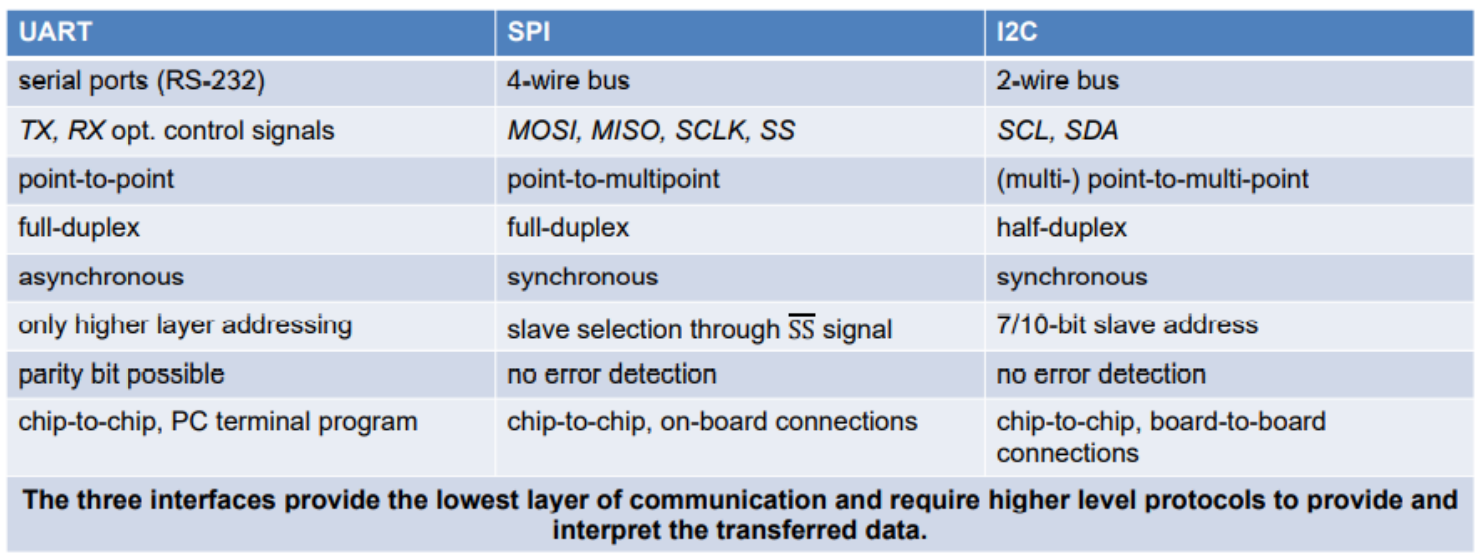
\includegraphics[width=\linewidth]{SDT_overview.png}

    \textbf{SPI - Serial Peripheral Interface}
    \begin{itemize}
        \item Master/slave architecture
        \item Synchronous full-duplex transmissions (MOSI, MISO) with shared clock
        \item Selection of device through Slave Select (SS) $\rightarrow$ multiple slaves possible, !! separate SS line for each slave
        \item no acknowledge, no error detection
        \item Clock signal (SCK) for synchronization: four mode $\rightarrow$ CPOL (clock polarity), CPHA (clock phase)
        \item High speed (up to 50+ Mbps)
    \end{itemize}
    \vspace{2mm}

    \textbf{UART - Universal Asynchronous Receiver Transmitter} (Serial Interface)
    \begin{itemize}
        \item Transmitter and receiver use diverging clocks
        \item Asynchronous (no shared clock) $\rightarrow$ synchronization using start and stop bits $\rightarrow$ overhead
        \item longer connections require line drivers $\rightarrow$ RS-232/RS-485
        \item simple wiring (2-3 wires)
        \item Moderate speed (up to ~5 Mbps)
    \end{itemize}
    \vspace{2mm}

    \textbf{I2C - Inter-Integrated Circuit}
    \begin{itemize}
        \item Multi-master, multi-slave
        \item Synchronous half-duplex transmission (SCL, SDA) with shared clock - SCL for synchronization
        \item 7-bit slave addresses
        \item Acknowledge, error detection
        \item Medium speed (100 kbps, 400 kbps, up to 5 Mbps)
    \end{itemize}
\end{concept}

\subsection{Protocol Comparison and Selection}

\begin{KR}{Selecting the Appropriate Serial Protocol}
\paragraph{Consider application requirements}
\begin{itemize}
    \item \textbf{Distance:}
    \begin{itemize}
        \item UART with RS-232 levels for longer distances
        \item SPI and I2C typically for on-board connections
    \end{itemize}
    \item \textbf{Speed:}
    \begin{itemize}
        \item SPI for highest speed requirements
        \item I2C for moderate speed with fewer pins
        \item UART for simpler, moderate speed connections
    \end{itemize}
    \item \textbf{Number of devices:}
    \begin{itemize}
        \item I2C for many devices on shared bus
        \item SPI for multiple devices but requires separate SS line for each
        \item UART typically for point-to-point (multiple UARTs needed for multiple devices)
    \end{itemize}
\end{itemize}

\paragraph{Evaluate protocol overhead}
\begin{itemize}
    \item \textbf{UART:} Start, stop, and optional parity bits and requires accurate clock timing
    \item \textbf{SPI:} Minimal protocol overhead, no addressing or acknowledgment
    \item \textbf{I2C:} Start/stop conditions, addressing, and acknowledgment $\rightarrow$ higher overhead, but better error detection
\end{itemize}

\paragraph{Consider hardware support}
\begin{itemize}
    \item Check if target microcontroller has hardware support for chosen protocol
    \item Consider available pins and alternate functions
    \item Evaluate available software libraries and drivers
    \item Consider power requirements (I2C has pull-up resistors that consume power)
\end{itemize}
\end{KR}

\begin{example}
Select the most appropriate serial protocol for each of the following applications:
\begin{enumerate}
    \item A system needs to connect a microcontroller to three temperature sensors. The sensors are low-cost devices that should be replaceable without redesigning the PCB. Data rate requirement is low.
    \item A data acquisition system needs to transfer large amounts of data from an ADC to a microcontroller at 20 Mbps.
    \item A microcontroller needs to communicate with a PC via USB port.
    \item A control system needs to connect to four different devices at varying distances up to 30 meters in an electrically noisy industrial environment.
\end{enumerate}
\paragraph{Solution:}

1. \textbf{I2C is most appropriate for the temperature sensors:}
   \begin{itemize}
     \item Multiple devices (three sensors) can be connected to the same two wires
     \item Each sensor has a unique address, making them individually addressable
     \item Low data rate requirement is well within I2C capabilities
     \item Sensors can be replaced without changing connections (as long as addresses are configured properly)
     \item Reduced pin count (only SCL and SDA) simplifies PCB design
   \end{itemize}
   \vspace{2mm}
2. \textbf{SPI is most appropriate for the high-speed ADC:}
   \begin{itemize}
     \item 20 Mbps data rate exceeds practical I2C speeds and most UART configurations
     \item SPI can easily handle 20+ Mbps with direct hardware support
     \item SPI's full-duplex capability allows simultaneous control and data transfer
     \item Minimal protocol overhead maximizes throughput for large data amounts
     \item Hardware-based chip select ensures proper timing for ADC operations
   \end{itemize}
   \vspace{2mm}
3. \textbf{UART is most appropriate for PC communication:}
   \begin{itemize}
     \item UART is the typical protocol used with USB-to-serial converter chips
     \item Simple point-to-point connection is sufficient for PC communication
     \item Standard baudrates (9600, 115200, etc.) are well-supported by PC software
     \item No need for extra clock signals simplifies interfacing with USB adapters
     \item Asynchronous nature accommodates timing differences between systems
   \end{itemize}
   \vspace{2mm}
4. \textbf{RS-485 (based on UART) is most appropriate for the industrial control system:}
   \begin{itemize}
     \item RS-485 extends UART to longer distances (up to 1200m)
     \item Differential signaling provides excellent noise immunity in industrial environments
     \item Multi-drop capability allows connection to four devices on a single bus
     \item Higher voltage levels offer better signal integrity over 30m distances
     \item Various data rates possible depending on cable length (up to 10 Mbps at shorter distances)
     \item Industry standard protocol with wide hardware support
   \end{itemize}
\end{example}







